\clearpage
\VerdierPhysicalPageAnchor{0084}%
\VerdierSemanticAnchor{ch1-3-1-2-phi-definition-continuation}
$\operatorname{tr}_1(C)$ 的下述态射：

\VerdierSemanticAnchor{ch1-3-1-2-phi-diagram}
\begin{equation*}
  \Phi(f)=(0,p(f),a(f))
  \qquad
  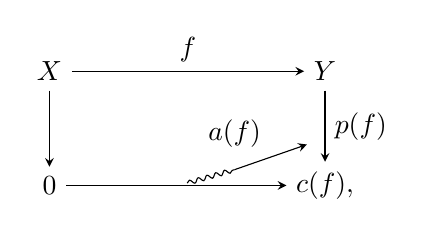
\begin{tikzpicture}[>=stealth,baseline=(current bounding box.center)]
    \node (X)  at (0,1.45) {$X$};
    \node (Y)  at (3.5,1.45) {$Y$};
    \node (Z)  at (0,0) {$0$};
    \node (Cf) at (3.5,0) {$c(f)\mathpunct{,}$};
    \draw[->] (X) -- node[above] {$f$} (Y);
    \draw[->] (X) -- (Z);
    \draw[->] (Y) -- node[right] {$p(f)$} (Cf);
    \draw[->] (Z) -- (Cf);
    \draw[decorate,decoration={snake,amplitude=0.8pt,segment length=3.3pt}]
      (1.75,0.03) -- (2.35,0.20);
    \draw[->] (2.35,0.20) -- node[above left] {$a(f)$} (3.27,0.52);
  \end{tikzpicture}
\end{equation*}

\VerdierSemanticAnchor{ch1-3-1-2-eq4}
\begin{equation}
  \begin{aligned}
    p(f)^i&=
      \begin{pmatrix}
        \operatorname{id}_{Y^i}\\[1mm]
        0
      \end{pmatrix}
      \colon Y^i\longrightarrow Y^i\oplus X^{i+1},\\[2mm]
    a(f)^i&=
      \begin{pmatrix}
        0\\[1mm]
        \operatorname{id}_{X^{i+1}}
      \end{pmatrix}
      \colon X^{i+1}\longrightarrow Y^i\oplus X^{i+1}.
  \end{aligned}
  \tag{3.1.2.4}
\end{equation}

\VerdierSemanticAnchor{ch1-3-1-2-phi-naturality}
直接计算表明，$\Phi$ 是从 $\operatorname{tr}_1(C)$ 的恒等函子到函子 $sc$
的一个函子态射。

\VerdierSemanticAnchor{ch1-3-1-3}
\noindent\textbf{命题 3.1.3.}\quad
\emph{态射 $\Phi$ 使映射锥函子成为函子 $s$ 的左伴随；即对
$\operatorname{tr}_1(C)$ 的任一对象 $X\xrightarrow{f}Y$ 和
$\operatorname{comp}(C)$ 的任一对象 $W$，由态射 $\Phi$ 定义的典范映射}

\VerdierSemanticAnchor{ch1-3-1-3-hom-isomorphism}
\begin{equation*}
  \operatorname{Hom}_{\operatorname{comp}(C)}(c(f),W)
  \longrightarrow
  \operatorname{Hom}_{\operatorname{tr}_1(C)}
    \bigl((X\xrightarrow{f}Y),sW\bigr)
\end{equation*}
\emph{是同构。}

\VerdierSemanticAnchor{ch1-3-1-3-verification}
验证留给读者。
\VerdierSemanticAnchor{ch1-3-1-3-s-fully-faithful}
注意，函子 $s$ 充分忠实，因而函子 $cs$ 典范同构于恒等函子。
\VerdierSemanticAnchor{ch1-3-1-3-cs-identity}
事实上，在所选的函子 $c$ 构造下，函子 $cs$ 等于恒等函子。
\VerdierSemanticAnchor{ch1-3-1-3-adjunction-reformulation}
(3.1.3) 的伴随性质也可表述如下：由函子定义的映射

\VerdierSemanticAnchor{ch1-3-1-3-c-hom-isomorphism}
\begin{equation*}
  c\colon
  \operatorname{Hom}_{\operatorname{tr}_1(C)}
    \bigl((X\xrightarrow{f}Y),sW\bigr)
  \longrightarrow
  \operatorname{Hom}_{\operatorname{comp}(C)}(c(f),W)
\end{equation*}
是同构。

\VerdierSemanticAnchor{ch1-3-1-4}
\noindent\textbf{3.1.4.}\quad
我们将在 $\operatorname{tr}_1(C)$ 中定义同伦的概念。设

\VerdierSemanticAnchor{ch1-3-1-4-homotopy-setup}
\begin{equation*}
  (g,h,a),(g',h',a')\colon
  (X\xrightarrow{f}Y)
  \rightrightarrows
  (X'\xrightarrow{f'}Y')
\end{equation*}
